\chapter{Conclusion}
\label{chap:conclusion}

\section{Conclusion}
\label{sec:conclusion}

This work presented the details of flexible FPGA-based SDR prototype. The
development of this setup was meant to be general and be used in both research
and academic environments. The process of implementing this setup involved a
large set of knowledges from distinct fields in telecommunications and embedded
systems, such as communication protocols, embedded programming, analog and
digital electronics and communication theory. Having such a setup for more
complex processes inside the LTE band saves a lot of time in development.

It was particularly demonstrated how the FMCOMMS2 board can be used. The FMCMMS2
board allows real-time and scalable change in parameters by software or hardware
signals, and it re-calibrates and reconfigures itself if needed so, which makes
a very good transceiver board to be used in a C-RAN capable radio unit.

This setup was extensively documented and can be used in digital communication
classes to show how a real radio front-end system is designed. In a setup such
as presented here it is possible to observe the real-world transmission behavior
of an arbitrary modulated waveform, this waveform can be generated in any
software or platform. This work also clarified how the data interface works and
how to work with different devices with different clock rates and it clarified
how to develop in such environment.

This work is also running in a microcontroller without any operating system,
which is a very interesting environment to understand computer hardware in a
low-level fashion. The study of the software in the processor can clarify some
aspects of design embedded systems.

Although the FMCOMMS2 and the FPGA operates on different clocks and no real
synchronization was implemented, this setup has the capability of transmitting
and receiving signals and reconfigure itself on real-time, which is one of the
requirements presented in Chapters \ref{chap:sdr} and \ref{chap:lte}.

\section{Future Works}
\label{sec:futurew}

In this work, there is no communication protocol between the FPGA (BBP) and the
external world other than the FMCCOMMS2. Such things are necessary to have a real
front-end but were outside the scope of this project which was just to evaluate a
setup for a scalable and dynamically configurable front-end.

The prototype developed in this work can be improved in terms of flexibility by
adding Ethernet connection driver in the FPGA, making it possible to receive
data from Ethernet and hand this data to the transceiver board following the
idea presented in the schematic \ref{fig:setupeth}. TIn order to do so,
particularly for synchronous transmission of data coming via Ethernet, proper
synchronization would be required. There would be some difficulty associated
with this improvement, mainly because the clock in which everything inside the
FPGA works is different from the AD9361 clock not only in frequency but in
phase, which can bring a lot of problems. However, there is the possibility of
feeding FMCCOMMS2 with an external clock which would increase its performance.

With Ethernet it would be possible to generate the modulated samples in an
external software (e.g. in a PC) and send them trough air, similar to what
GNURadio accomplishes when connected to an USRP. Additionally, it would be
possible to demodulate the received samples in the PC. Furthermore, there is the
possibility of introducing modulation and demodulation blocks in the FPGA
fabric. This would yield much better performance than the PC ones. Besides, with
partial reconfiguration there is the advantage of loading various schemes of
modulation/demodulation in the FPGA and switching between the schemes
on-the-fly. The Ethernet connection, is also very interesting for C-RAN
environment, because Ethernet is cheap and easy to implement.

\begin{figure}[htbp]
    \centering
    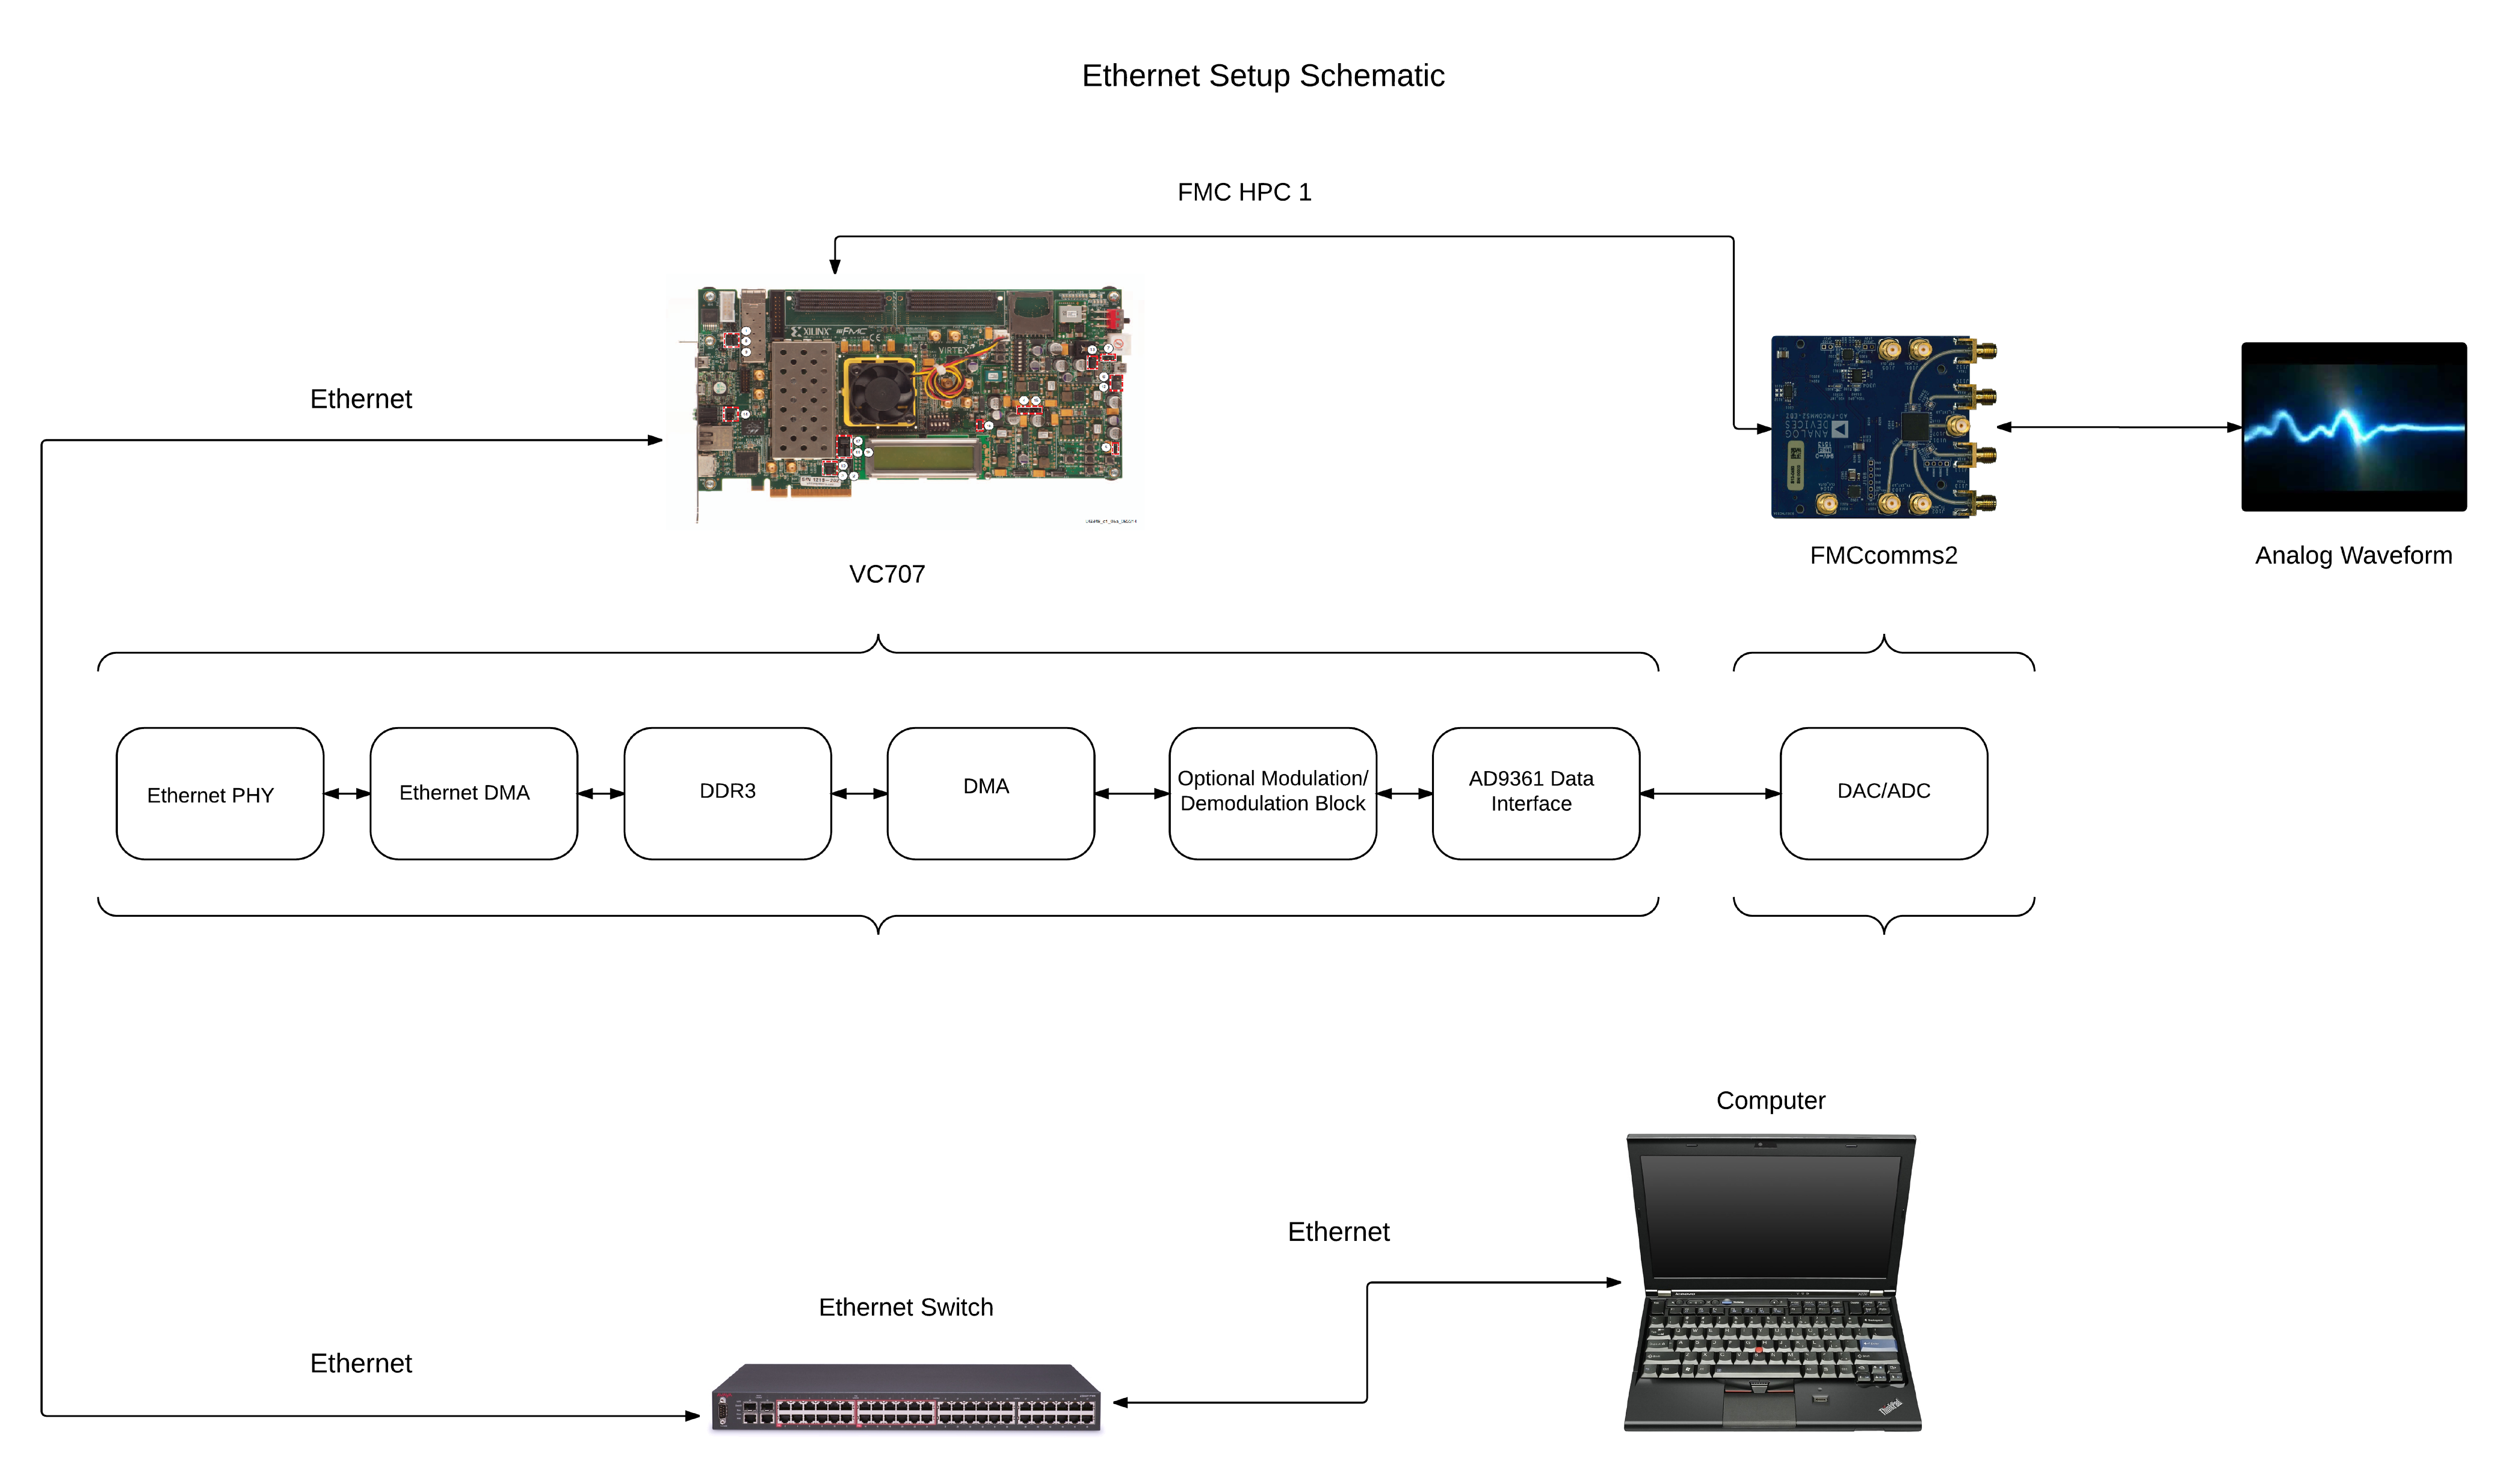
\includegraphics[width=0.95\textwidth]{./figures/eth_setup}
    \caption{ Setup enhanced with ethernet connection.
    \label{fig:setupeth}}
\end{figure}
